\documentclass{beamer}

% Requires the metropolis theme:
%   tlmgr install beamertheme-metropolis
% Or via your distro's package manager.
% Clean, modern, projection-friendly.
\usetheme{metropolis}

\usepackage{graphicx}
\usepackage{csquotes}
\usepackage{tikz}

% Adjust as needed for your projector environment
\metroset{block=fill}

\title{Updating Your Religion}
\author{Hans Halvorson}
\institute{Princeton University}
\date{Reunions 2026}

% ============================================================
\begin{document}
% ============================================================

\maketitle

%% where does science actually bear on religious beliefs?

% ------------------------------------------------------------
% SECTION 1: Introduction
% ------------------------------------------------------------

\section{Introduction}

\begin{frame}{Growing pains}
  I received a fundamentalist Christian worldview.\\[1em]
  
 My professors in college helped me to start updating my worldview.\\[1em]

 Data: the natural world, the claims of other human beings
\end{frame}

\begin{frame}{Overview}
  Does physics rule out human immortality? (Carroll's challenge)\\[1em]
  
  The limits of objective inquiry: what Møller and Kierkegaard teach us\\[1em]
  
  The danger of a quick fix: why NOMA fails both science and religion\\[1em]
  
  Status report: toward a worldview adequate for physics \emph{and} for persons
\end{frame}

% ------------------------------------------------------------
% SECTION 2: Does physics rule out immortality?
% ------------------------------------------------------------

\section{Does physics rule out immortality?}

\begin{frame}{Sean Carroll's argument}
  \begin{columns}[T]
    \begin{column}{0.55\textwidth}
      \vspace{0.5em}
      QFT gives a \textbf{complete inventory} of what exists at the energy scales relevant to human biology.\\[0.75em]
      If a soul interacted with the body, it would couple to known fields. Such a coupling would produce \textbf{detectable anomalies}. None are observed.
    \end{column}
    \begin{column}{0.40\textwidth}
      \centering
      
\includegraphics[height=0.35\textheight]{img/carroll.jpg}\\[0.5em]
      
\includegraphics[height=0.45\textheight]{img/carroll-book.jpg}
    \end{column}
  \end{columns}
\end{frame}

\begin{frame}{Letting science guide us}
  Germ theory replaced miasma theory. We do not believe bad air causes disease.\\[1em]
  Vaccines work. The science has settled the question, whatever traditional views may say.\\[1em]
  These are cases where an old view \textbf{must be given up because of science}.\\[1em]
  Carroll wants his argument to belong to this category. \textit{He may be right about the form of the argument.}
\end{frame}

\begin{frame}{Beating the atheist at his own game?}
  
  Some argue that the latest physics supports traditional religious doctrines:\\[0.75em]
  \begin{itemize}
    \item The fine-tuning argument
    \item Quantum mechanics and the soul
  \end{itemize}
  \vspace{0.75em} Both moves are suspicious for the same reason: they
  try to answer existential questions via objective inquiry.
\end{frame}

% ------------------------------------------------------------
% SECTION 3: The Danish rebellion against Hegel
% ------------------------------------------------------------

\section{The limits of objective inquiry}

\begin{frame}{An old argument in new dress}
  \begin{displayquote}
    \small Whoever is somewhat able to read between the lines in Hegel's writings will easily reach the inevitable conclusion that this philosopher holds the concept of personal immortality to be a notion with no reality at all.
  \end{displayquote}
  \vspace{0.5em}
  Sean Carroll is not the first to use the dominant scientific framework of his day in an argument against immortality.\\[0.75em]
  Left-wing Hegelians~--- e.g.\ Feuerbach, Strauss~--- made the same move in the 1830s and 40s: Hegel's System leaves no room for an immortal individual soul.\\[0.75em]
  Danish philosophers saw a flaw at the root of the Hegelian approach.\\[0.5em]
  \itshape Their lesson still applies.
\end{frame}

\begin{frame}{Poul Martin M\o{}ller (1794--1838)}
  \begin{columns}[T]
    \begin{column}{0.60\textwidth}
      \vspace{0.5em}
      \begin{displayquote}
        \small Those who ask for a demonstration of the reality of the doctrine of immortality and are unacquainted with the nature of science do not really know what they are asking for.
      \end{displayquote}
      \vspace{0.5em}
      Arguments \emph{for} and \emph{against} immortality fail for the \textbf{same reason}.\\[0.75em]
      Both sides treat immortality as an objective question~--- a fact to be settled from the outside.\\[0.75em]
      If the human subject doesn't participate in the infinite, then scientific results are insignificant.
    \end{column}
    \begin{column}{0.35\textwidth}
      
\includegraphics[height=0.40\textheight]{img/moller.jpg}\\[0.5em]
      
\includegraphics[height=0.50\textheight]{img/immortal.jpg}
    \end{column}
  \end{columns}
\end{frame}

\begin{frame}{S\o{}ren Kierkegaard (1813--1855)}
  \begin{columns}[T]
    \begin{column}{0.55\textwidth}
      \vspace{0.5em}
      \begin{displayquote}
        \small
        Objectively the question cannot be answered,
        because objectively it cannot be put.
      \end{displayquote}
      \vspace{0.75em}
      \normalsize
      Putting the subject in the background is a \textbf{methodological} demand~--- it is how science works.\\[0.75em]
      Carroll treats it as a \textbf{metaphysical} discovery: the subject simply doesn't matter.\\[0.75em]
      \itshape Mistaking a methodological idealization for a conclusion about reality.
    \end{column}
    \begin{column}{0.40\textwidth}
      
\includegraphics[width=\columnwidth]{img/kierkegaard.png}\\[0.5em]
      
\includegraphics[height=0.6\textheight]{img/postscript.jpg}
    \end{column}
  \end{columns}
\end{frame}

\begin{frame}{The view from nowhere}
  \begin{displayquote}
    \small I know that I have not found it in the System, where indeed it is also unreasonable to seek it; for, in a fantastic sense, all systematic thinking is \emph{sub specie aeterni}\ldots{} the question is about the immortality of a mortal, which is not answered by showing that the eternal is immortal.
  \end{displayquote}
  \vspace{0.75em}
  Kierkegaard's target: \textbf{Hegel's system}~--- thinking \emph{sub specie aeterni}, from the standpoint of eternity and the universal, where the existing individual simply disappears.\\[1em]
  Our target: \textbf{Physical theory}~--- a framework that likewise operates from nowhere in particular, after the subject has been removed.\\[1em]
  \large Hegel's aspirations were no different in principle than those of physics today. (Weinberg: \textit{Dreams of a Final Theory})
\end{frame}

% ------------------------------------------------------------
% SECTION 4: Danger: The doctrine of two truths
% ------------------------------------------------------------

\section{Temptation: Non-overlapping magisteria}

\begin{frame}{Gould's non-overlapping magisteria}
  \vspace{0.5em}
  \centering
  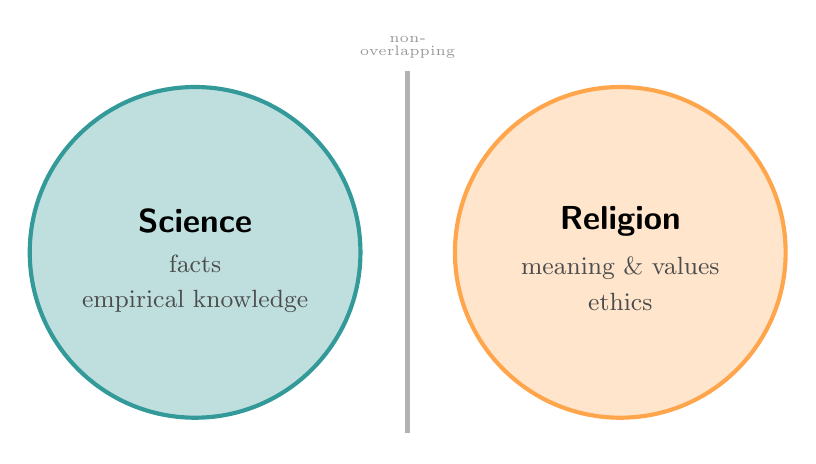
\begin{tikzpicture}[font=\sffamily]
    % Science circle
    \draw[fill=teal!25, draw=teal!80, line width=1.5pt]
      (-2.7, 0.4) circle (2.1cm);
    \node[align=center] at (-2.7, 0.8)
      {\large\textbf{Science}};
    \node[align=center, font=\small, text=black!70] at (-2.7, 0)
      {facts\\[0.2em]empirical knowledge};
    % Religion circle
    \draw[fill=orange!20, draw=orange!70, line width=1.5pt]
      (2.7, 0.4) circle (2.1cm);
    \node[align=center] at (2.7, 0.8)
      {\large\textbf{Religion}};
    \node[align=center, font=\small, text=black!70] at (2.7, 0)
      {meaning \& values\\[0.2em]ethics};
    % Wall
    \draw[line width=2pt, black!30] (0, -1.9) -- (0, 2.7);
    \node[font=\tiny, text=black!40, align=center] at (0, 3.0)
      {non-\\[-0.2em]overlapping};
  \end{tikzpicture}
\end{frame}

\begin{frame}{Rasmus Nielsen's failed attempt}
  Nielsen tried to wall off religious claims from scientific challenge entirely.\\[1em]
  \textbf{Hans Br\o{}chner's objection}: the partition thesis is self-undermining. The declaration that science and faith cannot touch each other is itself a philosophical claim~--- which Nielsen's own law forbids.\\[0.5em]
  \itshape You cannot step outside both domains to declare them non-overlapping.\\[1em]
  \upshape\textbf{NOMA is bad for religion}: a faith that rational inquiry cannot reach has abandoned \emph{fides quaerens intellectum}. Nielsen's faith is \textbf{static by design}.
\end{frame}

\begin{frame}{Analogy: Determinism and free will}
  %% SPEAK: NOMA's move --- like compatibilism in the free will debate ---
  %% partitions the domains to eliminate the conflict. Tidy. Widely accepted.
  \textbf{NOMA} = compatibilism applied to science and religion.\\[1em]
  %% SPEAK: But a science with no stake in self-understanding has no stake
  %% in the human project. Its only remaining motivation: control the world,
  %% extract material benefits. Might as well delegate to the AIs.
  \textbf{Science with no stake in the human project}\\becomes a tool of control and extraction.\\[1em]
  %% SPEAK: Gnōthi seauton. If science has nothing to say about seauton,
  %% all the worse for that science.
  \itshape Gn\={o}thi seauton: if science can't speak to \textit{seauton}, all the worse for that science.
\end{frame}

\begin{frame}{The cost of partition}
  \vspace{0.5em}
  \centering
  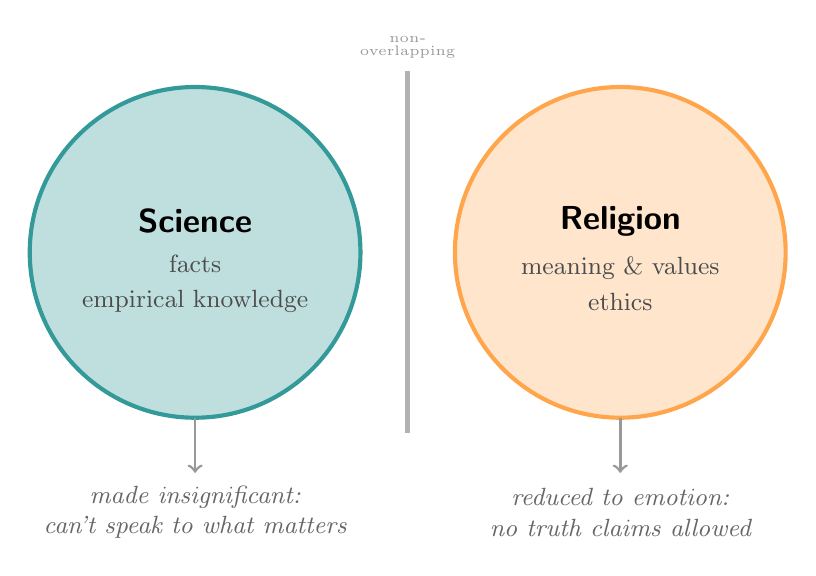
\begin{tikzpicture}[font=\sffamily]
    % Science circle
    \draw[fill=teal!25, draw=teal!80, line width=1.5pt]
      (-2.7, 0.4) circle (2.1cm);
    \node[align=center] at (-2.7, 0.8)
      {\large\textbf{Science}};
    \node[align=center, font=\small, text=black!70] at (-2.7, 0)
      {facts\\[0.2em]empirical knowledge};
    % Religion circle
    \draw[fill=orange!20, draw=orange!70, line width=1.5pt]
      (2.7, 0.4) circle (2.1cm);
    \node[align=center] at (2.7, 0.8)
      {\large\textbf{Religion}};
    \node[align=center, font=\small, text=black!70] at (2.7, 0)
      {meaning \& values\\[0.2em]ethics};
    % Wall
    \draw[line width=2pt, black!30] (0, -1.9) -- (0, 2.7);
    \node[font=\tiny, text=black!40, align=center] at (0, 3.0)
      {non-\\[-0.2em]overlapping};
    % Cost arrows and labels
    \draw[->, black!40, line width=1pt] (-2.7, -1.7) -- (-2.7, -2.4);
    \node[align=center, font=\small\itshape, text=black!60] at (-2.7, -2.9)
      {made insignificant:\\can't speak to what matters};
    \draw[->, black!40, line width=1pt] (2.7, -1.7) -- (2.7, -2.4);
    \node[align=center, font=\small\itshape, text=black!60] at (2.7, -2.9)
      {reduced to emotion:\\no truth claims allowed};
  \end{tikzpicture}
\end{frame}

% ------------------------------------------------------------
% SECTION 5: Status report
% ------------------------------------------------------------

\section{Status report}

\begin{frame}{A better path}
  Carroll: \textbf{begin without a subject}~--- the human being never enters the picture.\\[1em]
  %% SPEAK: Is there a more honest alternative? Yes --- and it has
  %% a distinguished history. Not religious apologists. Some of the
  %% most rigorous thinkers of the modern era.
  \textbf{The alternative}: begin with the human being doing science~--- for the human being.\\[1em]
  M\o{}ller $\to$ Kierkegaard $\to$ H\o{}ffding $\to$ Bohr:\\[0.5em]
  a tradition that never loses sight of the physicist as a person.
\end{frame}

\begin{frame}{Harald H\o{}ffding (1843--1931)}
  \begin{columns}[T]
    \begin{column}{0.55\textwidth}
      \vspace{0.5em}
      Our knowledge is always knowledge \emph{from somewhere, by someone}.\\[1em]
      This is not relativism. It is a constraint on what objectivity can mean.\\[1em]
      Took science seriously. Took religious orientation seriously. \textbf{Refused to dissolve the tension.}
    \end{column}
    \begin{column}{0.40\textwidth}
      
\includegraphics[height=0.45\textheight]{img/hoffding.jpg}
    \end{column}
  \end{columns}
\end{frame}

\begin{frame}{Niels Bohr (1885--1962)}
  \begin{columns}[T]
    \begin{column}{0.55\textwidth}
      \vspace{0.5em}
      \begin{displayquote}
        \small
        In the drama of existence we are ourselves both actors and spectators.
      \end{displayquote}
      \vspace{0.75em}
      \normalsize
      Not a retreat from objectivity~--- a more honest account of what objectivity can mean for a human inquirer.\\[0.75em]
      \small (Student of H\o{}ffding)
    \end{column}
    \begin{column}{0.40\textwidth}
      
\includegraphics[height=0.7\textheight]{img/bohr.jpg}
    \end{column}
  \end{columns}
\end{frame}

\begin{frame}{Bohr to his future mother-in-law}
  %% SPEAK: Written when Bohr left the Danish church, c. 1912.
  %% Carroll: value is a fiction. Bohr refuses this.
  %% The tradition goes all the way back to Møller:
  %% meaning in the world is real, even if it exceeds objective description.
  \vspace{0.5em}
  \begin{displayquote}
    \large
    ``But you must not think that I do not believe in anything at all;
    I believe that there is meaning in the world,
    a meaning that human beings cannot understand, but only sense.''
  \end{displayquote}
  \vspace{1em}
  \small\itshape Written when Bohr left the Danish church, c.\ 1912.
\end{frame}

\begin{frame}{An integrated worldview}
  %% SPEAK: Contrast with NOMA: not two separate domains,
  %% but one worldview with the self at the center.
  %% Physics guides metaphysics --- Carroll is right about that.
  %% But the path from physics to existential questions is long:
  %% it runs through metaphysics, ethics, the meaning of persons.
  %% Physics is at the periphery, not the center.
  %% Shimony: accommodate microphysics --- yes.
  %% But also accommodate persons.
  %% Van Fraassen (Princeton): critique of objectifying inquiry
  %% points in this direction.
  \centering
  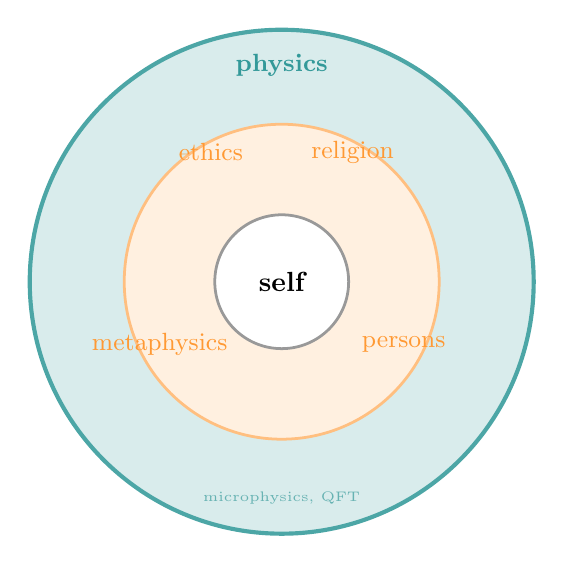
\begin{tikzpicture}[font=\sffamily]
    %% Outer ring: physics
    \draw[fill=teal!15, draw=teal!70, line width=1.5pt] (0,0) circle (3.2cm);
    \node[align=center, font=\small\bfseries, text=teal!80] at (0, 2.75)
      {physics};
    \node[align=center, font=\tiny, text=teal!60] at (0, -2.75)
      {microphysics, QFT};
    %% Middle ring: metaphysics, ethics, persons, religion
    \draw[fill=orange!12, draw=orange!50, line width=1pt] (0,0) circle (2.0cm);
    \node[align=center, font=\small, text=orange!80] at (-0.9, 1.65)
      {ethics};
    \node[align=center, font=\small, text=orange!80] at (0.9, 1.65)
      {religion};
    \node[align=center, font=\small, text=orange!80] at (-1.55, -0.8)
      {metaphysics};
    \node[align=center, font=\small, text=orange!80] at (1.55, -0.8)
      {persons};
    %% Center: self
    \draw[fill=white, draw=black!40, line width=1pt] (0,0) circle (0.85cm);
    \node[align=center, font=\normalsize\bfseries] at (0,0) {self};
  \end{tikzpicture}
\end{frame}

\begin{frame}{\textit{Gn\={o}thi seauton}}
  %% SPEAK: Most philosophers of physics are Fichtean dogmatists ---
  %% start from microphysics, attempt to save the manifest image.
  %% Taken to its conclusion: science as tool of control and material
  %% extraction, perfectly suited to techno-capitalism, with no
  %% internal resources to resist it.
  The dogmatist's move: start from microphysics.\\[1.25em]
  %% SPEAK: I've chosen the other tradition --- starting with Kant,
  %% really with Socrates. Not delivering results, but inviting
  %% you to stay in the dialogue.
  My choice: the tradition that starts with Socrates.\\[1.5em]
  \Large\textit{Gn\={o}thi seauton}\\[1.25em]
  \normalsize\itshape Stay in the dialogue.
\end{frame}

% ============================================================
\end{document}
% ============================================================

%%% Local Variables:
%%% mode: latex
%%% TeX-master: t
%%% End:
